\documentclass[11pt, letterpaper]{article}

% Fonts and Encoding
\usepackage[utf8]{inputenc}
\usepackage[T1]{fontenc}
\usepackage{lmodern} % High-quality Latin Modern vector font

% Math and Symbols
\usepackage{amsmath, amssymb, amsthm, amsfonts, mathrsfs, mathtools}

% Layout and Geometry
\usepackage{geometry}
\geometry{letterpaper, margin=1in}
\setlength{\parindent}{0pt}
\setlength{\parskip}{0.6em}

% Formatting and Graphics
\usepackage{graphicx, xcolor, enumitem, booktabs, array, tabularx}

% TikZ for Illustrations
\usepackage{tikz}
\usetikzlibrary{arrows.meta, positioning, shapes.geometric, calc, backgrounds, matrix}

% Clickable Links and TOC
\usepackage{hyperref}
\hypersetup{
    colorlinks=true,
    linkcolor=blue,
    filecolor=magenta,      
    urlcolor=cyan,
    pdftitle={Advanced Mathematics Topic},
}

% Theorem Environments
\newtheorem{theorem}{Theorem}[section]
\newtheorem{lemma}[theorem]{Lemma}
\newtheorem{proposition}[theorem]{Proposition}
\newtheorem{corollary}[theorem]{Corollary}
\theoremstyle{definition}
\newtheorem{definition}{Definition}[section]
\newtheorem{axiom}{Axiom}[section]
\newtheorem{example}{Example}[section]
\theoremstyle{remark}
\newtheorem{remark}{Remark}[section]

% Custom Commands (Enforced standard notation)
\newcommand{\R}{\mathbb{R}}
\newcommand{\N}{\mathbb{N}}
\newcommand{\Z}{\mathbb{Z}}
\newcommand{\Q}{\mathbb{Q}}
\newcommand{\E}{\mathbb{E}}
\newcommand{\Prob}{\mathbb{P}}
\newcommand{\F}{\mathcal{F}}

\begin{document}

\title{\textbf{Mastering the Gram-Schmidt Process and QR Factorization}}
\author{Tashfeen Omran}
\date{\today}
\maketitle

\tableofcontents
\newpage

\section{Part 1: Comprehensive Introduction, Context, and Prerequisites}

\subsection{Core Concepts}
The Gram-Schmidt process is a fundamental algorithm in linear algebra used to transform an arbitrary set of linearly independent vectors into an \textbf{orthogonal} (or \textbf{orthonormal}) basis that spans the exact same subspace. 

When working in $\R^n$, it is often highly advantageous to work with orthogonal vectors (vectors that are mutually perpendicular, meaning their dot product is zero). Orthogonal bases simplify computations immensely, particularly when finding coordinates of vectors, computing projections, or solving least-squares problems. If we further scale these orthogonal vectors so that each has a length (magnitude) of $1$, we obtain an \textbf{orthonormal basis}.

The Gram-Schmidt process also naturally leads to a matrix decomposition known as \textbf{QR Factorization}. Any matrix $A$ with linearly independent columns can be factored into $A = QR$, where $Q$ is a matrix with orthonormal columns and $R$ is an upper triangular invertible matrix.

\subsection{Intuition and Derivation}
The intuition behind the Gram-Schmidt process relies entirely on the concept of \textbf{orthogonal projection}. 
Imagine you have two linearly independent vectors, $x_1$ and $x_2$. 
1. We accept the first vector as it is: $v_1 = x_1$.
2. For the second vector, $x_2$, we want to keep only the ``part'' of $x_2$ that is perpendicular to $v_1$. We do this by finding the projection of $x_2$ onto $v_1$, and then \textit{subtracting} it from $x_2$. 
\[ v_2 = x_2 - \text{proj}_{v_1} x_2 \]
3. If we have a third vector $x_3$, we subtract its projection onto $v_1$ and its projection onto $v_2$. Because $v_1$ and $v_2$ are already orthogonal, these projections can be computed independently and subtracted.

\begin{center}
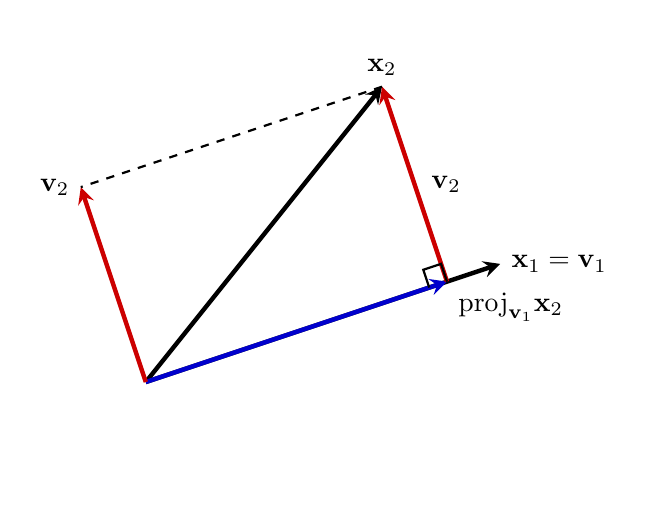
\begin{tikzpicture}[scale=1.5]
    % Background to ensure bounding box is clean
    \fill[white] (-1,-1) rectangle (4,3);
    
    % Vectors
    \draw[ultra thick, ->, >=stealth] (0,0) -- (3,1) node[right, text=black] {$\mathbf{x}_1 = \mathbf{v}_1$};
    \draw[ultra thick, ->, >=stealth] (0,0) -- (2,2.5) node[above, text=black] {$\mathbf{x}_2$};
    
    % Projection
    \draw[ultra thick, ->, >=stealth, blue!80!black] (0,0) -- (2.55, 0.85) node[below right, text=black] {$\text{proj}_{\mathbf{v}_1} \mathbf{x}_2$};
    
    % Orthogonal Component
    \draw[ultra thick, ->, >=stealth, red!80!black] (2.55, 0.85) -- (2,2.5) node[midway, right=2pt, text=black] {$\mathbf{v}_2$};
    
    % Shifted Orthogonal Component to origin
    \draw[ultra thick, ->, >=stealth, red!80!black] (0,0) -- (-0.55, 1.65) node[left, text=black] {$\mathbf{v}_2$};
    \draw[dashed, thick] (2,2.5) -- (-0.55, 1.65);
    
    % Right angle square
    \draw[thick] (2.4, 0.8) -- (2.35, 0.95) -- (2.5, 1.0) -- (2.55, 0.85);
\end{tikzpicture}
\end{center}

\subsection{Historical Context and Motivation}
The process is named after Jørgen Pedersen Gram and Erhard Schmidt, who popularized it in the late 19th and early 20th centuries, though it was previously discovered by Laplace and Cauchy. The primary motivation was to solve systems of linear equations and least-squares approximations more reliably. In numerical linear algebra, standard matrix inversion is highly susceptible to round-off errors. By orthogonalizing the system (via QR factorization), mathematicians created a numerically stable way to solve $Ax = b$ without ever computing $A^{-1}$.

\subsection{Key Formulas}
\begin{itemize}
    \item \textbf{Gram-Schmidt Orthogonalization:} Given a basis $\{x_1, \dots, x_p\}$, the orthogonal basis $\{v_1, \dots, v_p\}$ is:
    \begin{align*}
        v_1 &= x_1 \\
        v_2 &= x_2 - \frac{x_2 \cdot v_1}{v_1 \cdot v_1}v_1 \\
        v_3 &= x_3 - \frac{x_3 \cdot v_1}{v_1 \cdot v_1}v_1 - \frac{x_3 \cdot v_2}{v_2 \cdot v_2}v_2 \\
        &\vdots \\
        v_p &= x_p - \sum_{k=1}^{p-1} \frac{x_p \cdot v_k}{v_k \cdot v_k}v_k
    \end{align*}
    \item \textbf{Normalization:} To create an orthonormal basis $\{u_1, \dots, u_p\}$, scale each vector by its magnitude: $u_k = \frac{v_k}{\|v_k\|}$.
    \item \textbf{QR Factorization:} $A = QR$, where $Q = \begin{bmatrix} u_1 & u_2 & \dots & u_p \end{bmatrix}$ and $R = Q^T A$.
\end{itemize}

\subsection{Prerequisites}
To succeed in this topic, you must be fluent in:
1. \textbf{Dot Products:} Computing $u \cdot v = u_1v_1 + u_2v_2 + \dots + u_nv_n$.
2. \textbf{Vector Magnitudes:} Computing $\|v\| = \sqrt{v \cdot v}$.
3. \textbf{Matrix Multiplication:} Multiplying matrices and understanding transposes ($Q^T$).
4. \textbf{Linear Independence \& Span:} Understanding what constitutes a basis for a subspace.

\newpage
\section{Part 2: Detailed Homework Solutions}

\textit{Note: A strategic selection of problems has been chosen to cover every distinct problem archetype present in the text, ensuring full conceptual coverage without redundant repetition.}

\subsection{Type 1: Gram-Schmidt for 2 Vectors}

\textbf{Problem 1:} 
The given set is a basis for a subspace $W$. Use the Gram-Schmidt process to produce an orthogonal basis for $W$.
\[ x_1 = \begin{bmatrix} 3 \\ 0 \\ -1 \end{bmatrix}, \quad x_2 = \begin{bmatrix} 8 \\ 5 \\ -6 \end{bmatrix} \]

\textbf{Solution:}
\textbf{Step 1:} Set $v_1 = x_1$.
\[ v_1 = \begin{bmatrix} 3 \\ 0 \\ -1 \end{bmatrix} \]

\textbf{Step 2:} Compute $v_2 = x_2 - \frac{x_2 \cdot v_1}{v_1 \cdot v_1}v_1$.
First, we calculate the necessary dot products:
\begin{align*}
    x_2 \cdot v_1 &= (8)(3) + (5)(0) + (-6)(-1) = 24 + 0 + 6 = 30 \\
    v_1 \cdot v_1 &= (3)^2 + (0)^2 + (-1)^2 = 9 + 0 + 1 = 10
\end{align*}
Now, substitute these into the formula:
\begin{align*}
    v_2 &= \begin{bmatrix} 8 \\ 5 \\ -6 \end{bmatrix} - \frac{30}{10} \begin{bmatrix} 3 \\ 0 \\ -1 \end{bmatrix} \\ \relax
    &= \begin{bmatrix} 8 \\ 5 \\ -6 \end{bmatrix} - 3 \begin{bmatrix} 3 \\ 0 \\ -1 \end{bmatrix} \\ \relax
    &= \begin{bmatrix} 8 \\ 5 \\ -6 \end{bmatrix} - \begin{bmatrix} 9 \\ 0 \\ -3 \end{bmatrix} = \begin{bmatrix} -1 \\ 5 \\ -3 \end{bmatrix}
\end{align*}
\textbf{Final Answer:} The orthogonal basis is $\left\{ \begin{bmatrix} 3 \\ 0 \\ -1 \end{bmatrix}, \begin{bmatrix} -1 \\ 5 \\ -3 \end{bmatrix} \right\}$.

\vspace{1em}
\textbf{Problem 3:} 
Use the Gram-Schmidt process to produce an orthogonal basis for $W$.
\[ x_1 = \begin{bmatrix} 2 \\ -5 \\ 1 \end{bmatrix}, \quad x_2 = \begin{bmatrix} 4 \\ -1 \\ 2 \end{bmatrix} \]

\textbf{Solution:}
\textbf{Step 1:} Set $v_1 = x_1$.
\[ v_1 = \begin{bmatrix} 2 \\ -5 \\ 1 \end{bmatrix} \]

\textbf{Step 2:} Compute $v_2 = x_2 - \frac{x_2 \cdot v_1}{v_1 \cdot v_1}v_1$.
\begin{align*}
    x_2 \cdot v_1 &= (4)(2) + (-1)(-5) + (2)(1) = 8 + 5 + 2 = 15 \\
    v_1 \cdot v_1 &= (2)^2 + (-5)^2 + (1)^2 = 4 + 25 + 1 = 30
\end{align*}
Substitute into the formula:
\begin{align*}
    v_2 &= \begin{bmatrix} 4 \\ -1 \\ 2 \end{bmatrix} - \frac{15}{30} \begin{bmatrix} 2 \\ -5 \\ 1 \end{bmatrix} \\ \relax
    &= \begin{bmatrix} 4 \\ -1 \\ 2 \end{bmatrix} - \frac{1}{2} \begin{bmatrix} 2 \\ -5 \\ 1 \end{bmatrix} = \begin{bmatrix} 4 - 1 \\ -1 + 2.5 \\ 2 - 0.5 \end{bmatrix} = \begin{bmatrix} 3 \\ 1.5 \\ 1.5 \end{bmatrix}
\end{align*}
\textit{Optional but highly recommended step:} To avoid fractions, we can scale $v_2$ by multiplying it by $2$. Let $v_2' = 2v_2$.
\[ v_2' = \begin{bmatrix} 6 \\ 3 \\ 3 \end{bmatrix} \]
We can further divide by $3$ to get the simplest integer form: $v_2'' = \begin{bmatrix} 2 \\ 1 \\ 1 \end{bmatrix}$.
\textbf{Final Answer:} The orthogonal basis is $\left\{ \begin{bmatrix} 2 \\ -5 \\ 1 \end{bmatrix}, \begin{bmatrix} 2 \\ 1 \\ 1 \end{bmatrix} \right\}$.

\subsection{Type 2: Orthonormal Basis}

\textbf{Problem 7:} 
Find an orthonormal basis of the subspace spanned by the vectors in Exercise 3.

\textbf{Solution:}
From Exercise 3, we already have an orthogonal basis:
\[ v_1 = \begin{bmatrix} 2 \\ -5 \\ 1 \end{bmatrix}, \quad v_2 = \begin{bmatrix} 2 \\ 1 \\ 1 \end{bmatrix} \]
To make this an orthonormal basis, we must divide each vector by its magnitude.
\begin{align*}
    \|v_1\| &= \sqrt{2^2 + (-5)^2 + 1^2} = \sqrt{4 + 25 + 1} = \sqrt{30} \\
    u_1 &= \frac{1}{\sqrt{30}} \begin{bmatrix} 2 \\ -5 \\ 1 \end{bmatrix} = \begin{bmatrix} 2/\sqrt{30} \\ -5/\sqrt{30} \\ 1/\sqrt{30} \end{bmatrix}
\end{align*}
\begin{align*}
    \|v_2\| &= \sqrt{2^2 + 1^2 + 1^2} = \sqrt{4 + 1 + 1} = \sqrt{6} \\
    u_2 &= \frac{1}{\sqrt{6}} \begin{bmatrix} 2 \\ 1 \\ 1 \end{bmatrix} = \begin{bmatrix} 2/\sqrt{6} \\ 1/\sqrt{6} \\ 1/\sqrt{6} \end{bmatrix}
\end{align*}
\textbf{Final Answer:} The orthonormal basis is $\left\{ \begin{bmatrix} 2/\sqrt{30} \\ -5/\sqrt{30} \\ 1/\sqrt{30} \end{bmatrix}, \begin{bmatrix} 2/\sqrt{6} \\ 1/\sqrt{6} \\ 1/\sqrt{6} \end{bmatrix} \right\}$.

\subsection{Type 3: Gram-Schmidt for 3 Vectors in Higher Dimensions}

\textbf{Problem 9:} 
Find an orthogonal basis for the column space of the matrix:
\[ \begin{bmatrix} 3 & -5 & 1 \\ 1 & 1 & 1 \\ -1 & 5 & -2 \\ 3 & -7 & 8 \end{bmatrix} \]

\textbf{Solution:}
Let the columns be $x_1, x_2, x_3$.
\textbf{Step 1:} $v_1 = x_1 = \begin{bmatrix} 3 \\ 1 \\ -1 \\ 3 \end{bmatrix}$.

\textbf{Step 2:} $v_2 = x_2 - \frac{x_2 \cdot v_1}{v_1 \cdot v_1}v_1$.
\begin{align*}
    x_2 \cdot v_1 &= (-5)(3) + (1)(1) + (5)(-1) + (-7)(3) = -15 + 1 - 5 - 21 = -40 \\
    v_1 \cdot v_1 &= 3^2 + 1^2 + (-1)^2 + 3^2 = 9 + 1 + 1 + 9 = 20
\end{align*}
\begin{align*}
    v_2 &= \begin{bmatrix} -5 \\ 1 \\ 5 \\ -7 \end{bmatrix} - \frac{-40}{20} \begin{bmatrix} 3 \\ 1 \\ -1 \\ 3 \end{bmatrix} \\ \relax
    &= \begin{bmatrix} -5 \\ 1 \\ 5 \\ -7 \end{bmatrix} + 2 \begin{bmatrix} 3 \\ 1 \\ -1 \\ 3 \end{bmatrix} = \begin{bmatrix} -5 + 6 \\ 1 + 2 \\ 5 - 2 \\ -7 + 6 \end{bmatrix} = \begin{bmatrix} 1 \\ 3 \\ 3 \\ -1 \end{bmatrix}
\end{align*}

\textbf{Step 3:} $v_3 = x_3 - \frac{x_3 \cdot v_1}{v_1 \cdot v_1}v_1 - \frac{x_3 \cdot v_2}{v_2 \cdot v_2}v_2$.
\begin{align*}
    x_3 \cdot v_1 &= (1)(3) + (1)(1) + (-2)(-1) + (8)(3) = 3 + 1 + 2 + 24 = 30 \\
    x_3 \cdot v_2 &= (1)(1) + (1)(3) + (-2)(3) + (8)(-1) = 1 + 3 - 6 - 8 = -10 \\
    v_2 \cdot v_2 &= 1^2 + 3^2 + 3^2 + (-1)^2 = 1 + 9 + 9 + 1 = 20
\end{align*}
\begin{align*}
    v_3 &= \begin{bmatrix} 1 \\ 1 \\ -2 \\ 8 \end{bmatrix} - \frac{30}{20} \begin{bmatrix} 3 \\ 1 \\ -1 \\ 3 \end{bmatrix} - \frac{-10}{20} \begin{bmatrix} 1 \\ 3 \\ 3 \\ -1 \end{bmatrix} \\ \relax
    &= \begin{bmatrix} 1 \\ 1 \\ -2 \\ 8 \end{bmatrix} - \begin{bmatrix} 4.5 \\ 1.5 \\ -1.5 \\ 4.5 \end{bmatrix} + \begin{bmatrix} 0.5 \\ 1.5 \\ 1.5 \\ -0.5 \end{bmatrix} = \begin{bmatrix} 1 - 4.5 + 0.5 \\ 1 - 1.5 + 1.5 \\ -2 + 1.5 + 1.5 \\ 8 - 4.5 - 0.5 \end{bmatrix} = \begin{bmatrix} -3 \\ 1 \\ 1 \\ 3 \end{bmatrix}
\end{align*}
\textbf{Final Answer:} The orthogonal basis is $\left\{ \begin{bmatrix} 3 \\ 1 \\ -1 \\ 3 \end{bmatrix}, \begin{bmatrix} 1 \\ 3 \\ 3 \\ -1 \end{bmatrix}, \begin{bmatrix} -3 \\ 1 \\ 1 \\ 3 \end{bmatrix} \right\}$.

\vspace{1em}
\textbf{Problem 11:} 
Find an orthogonal basis for the column space of the matrix:
\[ \begin{bmatrix} 1 & 2 & 5 \\ -1 & 1 & -4 \\ -1 & 4 & -3 \\ 1 & -4 & 7 \\ 1 & 2 & 1 \end{bmatrix} \]

\textbf{Solution:}
Let the columns be $x_1, x_2, x_3$.
\textbf{Step 1:} $v_1 = x_1 = \begin{bmatrix} 1 \\ -1 \\ -1 \\ 1 \\ 1 \end{bmatrix}$. $v_1 \cdot v_1 = 1 + 1 + 1 + 1 + 1 = 5$.

\textbf{Step 2:} $v_2 = x_2 - \frac{x_2 \cdot v_1}{v_1 \cdot v_1}v_1$.
\[ x_2 \cdot v_1 = (2)(1) + (1)(-1) + (4)(-1) + (-4)(1) + (2)(1) = 2 - 1 - 4 - 4 + 2 = -5 \]
\[ v_2 = \begin{bmatrix} 2 \\ 1 \\ 4 \\ -4 \\ 2 \end{bmatrix} - \frac{-5}{5} \begin{bmatrix} 1 \\ -1 \\ -1 \\ 1 \\ 1 \end{bmatrix} = \begin{bmatrix} 2 \\ 1 \\ 4 \\ -4 \\ 2 \end{bmatrix} + \begin{bmatrix} 1 \\ -1 \\ -1 \\ 1 \\ 1 \end{bmatrix} = \begin{bmatrix} 3 \\ 0 \\ 3 \\ -3 \\ 3 \end{bmatrix} \]
\textit{Scale $v_2$ to simplify:} Let $v_2' = \frac{1}{3}v_2 = \begin{bmatrix} 1 \\ 0 \\ 1 \\ -1 \\ 1 \end{bmatrix}$. $v_2' \cdot v_2' = 1 + 0 + 1 + 1 + 1 = 4$.

\textbf{Step 3:} $v_3 = x_3 - \frac{x_3 \cdot v_1}{v_1 \cdot v_1}v_1 - \frac{x_3 \cdot v_2'}{v_2' \cdot v_2'}v_2'$.
\begin{align*}
    x_3 \cdot v_1 &= (5)(1) + (-4)(-1) + (-3)(-1) + (7)(1) + (1)(1) = 5 + 4 + 3 + 7 + 1 = 20 \\
    x_3 \cdot v_2' &= (5)(1) + (-4)(0) + (-3)(1) + (7)(-1) + (1)(1) = 5 + 0 - 3 - 7 + 1 = -4
\end{align*}
\begin{align*}
    v_3 &= \begin{bmatrix} 5 \\ -4 \\ -3 \\ 7 \\ 1 \end{bmatrix} - \frac{20}{5} \begin{bmatrix} 1 \\ -1 \\ -1 \\ 1 \\ 1 \end{bmatrix} - \frac{-4}{4} \begin{bmatrix} 1 \\ 0 \\ 1 \\ -1 \\ 1 \end{bmatrix} \\ \relax
    &= \begin{bmatrix} 5 \\ -4 \\ -3 \\ 7 \\ 1 \end{bmatrix} - 4 \begin{bmatrix} 1 \\ -1 \\ -1 \\ 1 \\ 1 \end{bmatrix} + \begin{bmatrix} 1 \\ 0 \\ 1 \\ -1 \\ 1 \end{bmatrix} = \begin{bmatrix} 5 - 4 + 1 \\ -4 + 4 + 0 \\ -3 + 4 + 1 \\ 7 - 4 - 1 \\ 1 - 4 + 1 \end{bmatrix} = \begin{bmatrix} 2 \\ 0 \\ 2 \\ 2 \\ -2 \end{bmatrix}
\end{align*}
\textit{Scale $v_3$ to simplify:} Let $v_3' = \frac{1}{2}v_3 = \begin{bmatrix} 1 \\ 0 \\ 1 \\ 1 \\ -1 \end{bmatrix}$.
\textbf{Final Answer:} The orthogonal basis is $\left\{ \begin{bmatrix} 1 \\ -1 \\ -1 \\ 1 \\ 1 \end{bmatrix}, \begin{bmatrix} 1 \\ 0 \\ 1 \\ -1 \\ 1 \end{bmatrix}, \begin{bmatrix} 1 \\ 0 \\ 1 \\ 1 \\ -1 \end{bmatrix} \right\}$.

\subsection{Type 4: QR Factorization}

\textbf{Problem 13:} 
The columns of $Q$ were obtained by applying the Gram-Schmidt process to the columns of $A$. Find an upper triangular matrix $R$ such that $A = QR$.
\[ A = \begin{bmatrix} 5 & 9 \\ 1 & 7 \\ -3 & -5 \\ 1 & 5 \end{bmatrix}, \quad Q = \begin{bmatrix} 5/6 & -1/6 \\ 1/6 & 5/6 \\ -3/6 & 1/6 \\ 1/6 & 3/6 \end{bmatrix} \]

\textbf{Solution:}
Since $Q$ has orthonormal columns, $Q^T Q = I$. We can find $R$ by left-multiplying $A = QR$ by $Q^T$:
\[ Q^T A = Q^T Q R = I R = R \]
So, $R = Q^T A$.
\[ R = \begin{bmatrix} 5/6 & 1/6 & -3/6 & 1/6 \\ -1/6 & 5/6 & 1/6 & 3/6 \end{bmatrix} \begin{bmatrix} 5 & 9 \\ 1 & 7 \\ -3 & -5 \\ 1 & 5 \end{bmatrix} \]
Compute the entries of $R$:
\begin{align*}
    r_{11} &= \frac{1}{6} \big( (5)(5) + (1)(1) + (-3)(-3) + (1)(1) \big) = \frac{25 + 1 + 9 + 1}{6} = \frac{36}{6} = 6 \\
    r_{12} &= \frac{1}{6} \big( (5)(9) + (1)(7) + (-3)(-5) + (1)(5) \big) = \frac{45 + 7 + 15 + 5}{6} = \frac{72}{6} = 12 \\
    r_{21} &= \frac{1}{6} \big( (-1)(5) + (5)(1) + (1)(-3) + (3)(1) \big) = \frac{-5 + 5 - 3 + 3}{6} = 0 \quad \text{(Expected, } R \text{ is upper triangular)} \\
    r_{22} &= \frac{1}{6} \big( (-1)(9) + (5)(7) + (1)(-5) + (3)(5) \big) = \frac{-9 + 35 - 5 + 15}{6} = \frac{36}{6} = 6
\end{align*}
\textbf{Final Answer:} $R = \begin{bmatrix} 6 & 12 \\ 0 & 6 \end{bmatrix}$.

\vspace{1em}
\textbf{Problem 15:} 
Find a QR factorization of the matrix in Exercise 11.

\textbf{Solution:}
From Exercise 11, we have the orthogonal basis for the columns of $A$:
\[ v_1 = \begin{bmatrix} 1 \\ -1 \\ -1 \\ 1 \\ 1 \end{bmatrix}, \quad v_2' = \begin{bmatrix} 1 \\ 0 \\ 1 \\ -1 \\ 1 \end{bmatrix}, \quad v_3' = \begin{bmatrix} 1 \\ 0 \\ 1 \\ 1 \\ -1 \end{bmatrix} \]
\textbf{Step 1: Construct $Q$ by normalizing these vectors.}
\begin{align*}
    \|v_1\| &= \sqrt{5} \implies u_1 = \frac{1}{\sqrt{5}} \begin{bmatrix} 1 \\ -1 \\ -1 \\ 1 \\ 1 \end{bmatrix} \\
    \|v_2'\| &= \sqrt{1+0+1+1+1} = \sqrt{4} = 2 \implies u_2 = \frac{1}{2} \begin{bmatrix} 1 \\ 0 \\ 1 \\ -1 \\ 1 \end{bmatrix} \\
    \|v_3'\| &= \sqrt{1+0+1+1+1} = \sqrt{4} = 2 \implies u_3 = \frac{1}{2} \begin{bmatrix} 1 \\ 0 \\ 1 \\ 1 \\ -1 \end{bmatrix}
\end{align*}
\[ Q = \begin{bmatrix} 1/\sqrt{5} & 1/2 & 1/2 \\ -1/\sqrt{5} & 0 & 0 \\ -1/\sqrt{5} & 1/2 & 1/2 \\ 1/\sqrt{5} & -1/2 & 1/2 \\ 1/\sqrt{5} & 1/2 & -1/2 \end{bmatrix} \]

\textbf{Step 2: Construct $R$ using $R = Q^T A$.}
Since $R$ is upper triangular, $r_{ij} = 0$ for $i > j$. We compute $r_{ij} = u_i \cdot x_j$ for $i \leq j$.
\begin{align*}
    r_{11} &= u_1 \cdot x_1 = \frac{1}{\sqrt{5}}(1 + 1 + 1 + 1 + 1) = \frac{5}{\sqrt{5}} = \sqrt{5} \\
    r_{12} &= u_1 \cdot x_2 = \frac{1}{\sqrt{5}}(2 - 1 - 4 - 4 + 2) = \frac{-5}{\sqrt{5}} = -\sqrt{5} \\
    r_{13} &= u_1 \cdot x_3 = \frac{1}{\sqrt{5}}(5 + 4 + 3 + 7 + 1) = \frac{20}{\sqrt{5}} = 4\sqrt{5} \\
    r_{22} &= u_2 \cdot x_2 = \frac{1}{2}(2 + 0 + 4 + 4 + 2) = \frac{12}{2} = 6 \\
    r_{23} &= u_2 \cdot x_3 = \frac{1}{2}(5 + 0 - 3 - 7 + 1) = \frac{-4}{2} = -2 \\
    r_{33} &= u_3 \cdot x_3 = \frac{1}{2}(5 + 0 - 3 + 7 - 1) = \frac{8}{2} = 4
\end{align*}
\textbf{Final Answer:} 
\[ Q = \begin{bmatrix} 1/\sqrt{5} & 1/2 & 1/2 \\ -1/\sqrt{5} & 0 & 0 \\ -1/\sqrt{5} & 1/2 & 1/2 \\ 1/\sqrt{5} & -1/2 & 1/2 \\ 1/\sqrt{5} & 1/2 & -1/2 \end{bmatrix}, \quad R = \begin{bmatrix} \sqrt{5} & -\sqrt{5} & 4\sqrt{5} \\ 0 & 6 & -2 \\ 0 & 0 & 4 \end{bmatrix} \]

\subsection{Type 5: Conceptual True/False and Proofs}

\textbf{Problem 17:} (T/F) If $\{v_1, v_2, v_3\}$ is an orthogonal basis for $W$, then multiplying $v_3$ by a scalar $c$ gives a new orthogonal basis $\{v_1, v_2, cv_3\}$.
\textbf{Solution:} \textbf{False.} If $c = 0$, the vector becomes the zero vector. A basis cannot contain the zero vector because it would no longer be linearly independent. (If the statement specified $c \neq 0$, it would be true).

\vspace{1em}
\textbf{Problem 18:} (T/F) If $W = \text{Span}\{x_1, x_2, x_3\}$ with $\{x_1, x_2, x_3\}$ linearly independent, and if $\{v_1, v_2, v_3\}$ is an orthogonal set in $W$, then $\{v_1, v_2, v_3\}$ is a basis for $W$.
\textbf{Solution:} \textbf{False.} An orthogonal set can contain the zero vector. To be a basis for a 3-dimensional space, the set must contain exactly 3 \textit{nonzero} orthogonal vectors.

\vspace{1em}
\textbf{Problem 21:} (T/F) If $A = QR$, where $Q$ has orthonormal columns, then $R = Q^T A$.
\textbf{Solution:} \textbf{True.} Because $Q$ has orthonormal columns, $Q^T Q = I$. Left-multiplying both sides of $A = QR$ by $Q^T$ yields $Q^T A = Q^T Q R = I R = R$.

\vspace{1em}
\textbf{Problem 23:} Suppose $A = QR$, where $Q$ is $m \times n$ and $R$ is $n \times n$. Show that if the columns of $A$ are linearly independent, then $R$ must be invertible.
\textbf{Solution:} 
To show $R$ is invertible, we must show that the homogeneous equation $Rx = 0$ has only the trivial solution $x = 0$.
Assume $Rx = 0$. 
Left-multiply both sides by $Q$:
\[ Q(Rx) = Q(0) \implies (QR)x = 0 \implies Ax = 0 \]
We are given that the columns of $A$ are linearly independent. By definition, if the columns of $A$ are linearly independent, the equation $Ax = 0$ has only the trivial solution $x = 0$.
Therefore, $Rx = 0$ implies $x = 0$. By the Invertible Matrix Theorem, $R$ must be invertible.

\newpage
\section{Part 3: In-Depth Analysis of Problems and Techniques}

\subsection{A) Problem Types and General Approach}

\renewcommand{\arraystretch}{1.5}
\begin{tabularx}{\textwidth}{>{\raggedright\arraybackslash}p{4cm} X}
\toprule
\textbf{Problem Type} & \textbf{General Strategy} \\
\midrule
\textbf{Gram-Schmidt (2 or 3 Vectors)} & Apply the iterative projection formula. Always set $v_1 = x_1$. For subsequent vectors, subtract the projection of $x_k$ onto all previously found \textit{orthogonal} vectors $v_1, \dots, v_{k-1}$. \\
\addlinespace[4pt]
\textbf{Orthonormalization} & First, complete the standard Gram-Schmidt process to find the orthogonal basis $\{v_1, \dots, v_p\}$. Then, divide each vector by its magnitude: $u_k = v_k / \|v_k\|$. \\
\addlinespace[4pt]
\textbf{Finding $R$ given $A$ and $Q$} & Do not re-run the Gram-Schmidt process. Exploit the property of orthonormal matrices ($Q^T Q = I$). Simply compute the matrix multiplication $R = Q^T A$. \\
\addlinespace[4pt]
\textbf{Full QR Factorization} & 1. Run Gram-Schmidt on columns of $A$. \newline 2. Normalize to get $Q$. \newline 3. Compute $R = Q^T A$ (or build $R$ using the dot products $u_i \cdot x_j$ calculated during step 2). \\
\bottomrule
\end{tabularx}

\subsection{B) Key Algebraic and Calculus Manipulations}

\begin{itemize}
    \item \textbf{The Scaling Trick (Crucial for Speed):} In Problems 3 and 11, the raw Gram-Schmidt formula produced vectors with fractions (e.g., $v_2 = [3, 1.5, 1.5]^T$). Because we only care about the \textit{direction} for orthogonality, we can multiply the entire vector by a scalar (like $2$) to clear the denominators before using it in the next step. This prevents a cascade of messy fraction arithmetic.
    \item \textbf{Exploiting Upper Triangularity:} When computing $R = Q^T A$, we know theoretically that $R$ must be upper triangular. This means for any $i > j$, the dot product $q_i \cdot a_j$ \textit{must} be zero. You can use this as a built-in error check during exams. If $q_2 \cdot a_1 \neq 0$, you made an arithmetic mistake in finding $Q$.
    \item \textbf{Matrix Multiplication as Dot Products:} Recognizing that the entry $r_{ij}$ in $R = Q^T A$ is exactly the dot product of the $i$-th column of $Q$ and the $j$-th column of $A$.
\end{itemize}

\newpage
\section{Part 4: "Cheatsheet" and Tips for Success}

\subsection{Summary of Important Formulas}
\renewcommand{\arraystretch}{1.5}
\begin{tabularx}{\textwidth}{>{\raggedright\arraybackslash}p{5cm} >{$\displaystyle}X<{$}}
\toprule
\textbf{Concept} & \text{\textbf{Formula}} \\
\midrule
\textbf{Projection of $x$ onto $v$} & \text{proj}_{v} x = \frac{x \cdot v}{v \cdot v} v \\
\addlinespace[4pt]
\textbf{Gram-Schmidt Iteration} & v_k = x_k - \sum_{j=1}^{k-1} \frac{x_k \cdot v_j}{v_j \cdot v_j} v_j \\
\addlinespace[4pt]
\textbf{Normalization} & u_k = \frac{v_k}{\|v_k\|} \\
\addlinespace[4pt]
\textbf{QR Factorization} & A = QR \quad \text{where} \quad R = Q^T A \\
\bottomrule
\end{tabularx}

\subsection{Cheats, Tricks, and Shortcuts}
\begin{itemize}
    \item \textbf{Scale Immediately:} The moment a $v_k$ vector yields fractions, multiply it by the least common multiple of the denominators. Use this new scaled vector for all future dot products.
    \item \textbf{Build $R$ on the Fly:} The entries of $R$ are just the coefficients used in the Gram-Schmidt process, adjusted for normalization. Specifically, $r_{ij} = u_i \cdot x_j$. You already compute the numerators of these fractions during Gram-Schmidt!
    \item \textbf{Check Orthogonality Early:} After finding $v_2$, immediately check if $v_1 \cdot v_2 = 0$. If it doesn't, stop. Do not proceed to $v_3$, because the error will compound and ruin the rest of the problem.
\end{itemize}

\subsection{Common Pitfalls and Traps}
\begin{itemize}
    \item \textbf{The "Original Vector" Trap:} When computing $v_3$, students often accidentally project $x_3$ onto $x_1$ and $x_2$ instead of the orthogonalized vectors $v_1$ and $v_2$. The formula strictly requires projecting onto the $v$'s.
    \item \textbf{Forgetting to Normalize for $Q$:} The matrix $Q$ in a QR factorization must have \textit{orthonormal} columns, not just orthogonal. If you forget to divide by the magnitudes, your $Q$ is wrong, and $Q^T Q \neq I$.
    \item \textbf{Square Root Arithmetic:} When normalizing, leave the magnitudes as $1/\sqrt{c}$ outside the vector until the very end. Distributing the square root into every component early makes matrix multiplication for $R$ visually overwhelming.
\end{itemize}

\newpage
\section{Part 5: Conceptual Synthesis and The "Big Picture"}

\subsection{A) Thematic Connections}
The core theme of the Gram-Schmidt process is \textbf{orthogonal decomposition}—breaking down a complex, overlapping system into independent, non-overlapping components. 
This theme appears everywhere in mathematics:
*   \textbf{Calculus/Physics:} Decomposing a force vector into horizontal ($x$) and vertical ($y$) components.
*   \textbf{Fourier Series:} Decomposing a complex periodic wave into a sum of mutually orthogonal sine and cosine waves. In the space of continuous functions, sine and cosine act exactly like the orthogonal vectors $v_1, v_2, \dots$ generated by Gram-Schmidt.

\subsection{B) Forward and Backward Links}
\textbf{Backward Links:} This topic is the logical culmination of basic vector operations. It takes the dot product (a measure of parallel-ness) and vector projection, and loops them into an algorithm to systematically eliminate parallel components.

\textbf{Forward Links:} Gram-Schmidt is the bedrock for advanced linear algebra and numerical analysis. 
1. \textbf{Least Squares:} In Section 6.5, you will solve $Ax = b$ when no solution exists by projecting $b$ onto the column space of $A$. Orthogonal bases make this projection trivial.
2. \textbf{Eigenvalue Algorithms:} The QR algorithm (iteratively factoring $A_k = Q_k R_k$ and multiplying $A_{k+1} = R_k Q_k$) is the standard method computers use to find eigenvalues of large matrices.
3. \textbf{Spectral Theorem \& SVD:} Understanding orthonormal bases is required to understand the Singular Value Decomposition (SVD), arguably the most important theorem in applied linear algebra.

\section{Part 6: Abstract Real-World Modeling (AI, ML, \& Quant Finance)}

\subsection{A) Concrete Scenarios}
1. \textbf{Quantitative Finance (Risk Factor Orthogonalization):} In multi-factor models (like the Fama-French model), risk factors (e.g., market risk, size, value) are often correlated. Quants use Gram-Schmidt (or PCA, its statistical cousin) to orthogonalize these factors. This creates a set of uncorrelated synthetic assets, allowing portfolio managers to hedge specific risks without accidentally increasing exposure to others.
2. \textbf{Machine Learning (Numerically Stable OLS):} In Ordinary Least Squares (OLS) regression, the theoretical solution is $\beta = (X^T X)^{-1} X^T y$. However, if features are highly correlated, $X^T X$ becomes nearly singular (high condition number), and inverting it causes catastrophic floating-point overflow. ML libraries (like scikit-learn) use QR factorization to solve this stably.

\subsection{B) Model Problem Setup: Stable OLS via QR Factorization}
Let us formulate the OLS problem using QR factorization for a Machine Learning application.
\textbf{State Space \& Variables:}
Let $X \in \R^{m \times n}$ be a design matrix of $m$ observations and $n$ features, where $m > n$ and $\text{rank}(X) = n$. Let $y \in \R^m$ be the target vector. We assume a linear data-generating process $y = X\beta + \epsilon$, where $\epsilon \sim \mathcal{N}(0, \sigma^2 I)$.

\textbf{Optimization Problem:}
We seek to minimize the Residual Sum of Squares (RSS) loss function:
\[ \mathcal{L}(\beta) = \| y - X\beta \|_2^2 \]

\textbf{Theoretical Framework (QR Approach):}
Instead of solving the normal equations $X^T X \beta = X^T y$, we apply the Gram-Schmidt process to factor $X = QR$, where $Q \in \R^{m \times n}$ has orthonormal columns ($Q^T Q = I_n$) and $R \in \R^{n \times n}$ is upper triangular and invertible.
Substitute $X = QR$ into the loss function:
\[ \mathcal{L}(\beta) = \| y - QR\beta \|_2^2 \]
Because multiplying by an orthogonal matrix (or projecting onto its span) preserves the Euclidean norm for vectors in that span, the least-squares solution satisfies:
\[ R\beta = Q^T y \]
Since $R$ is upper triangular, we do not need to compute a matrix inverse. We solve for $\beta$ using \textbf{backward substitution}, starting from $\beta_n$ up to $\beta_1$. This algorithm requires $\mathcal{O}(mn^2)$ operations and is highly robust against multicollinearity in the feature matrix $X$.

\newpage
\section{Part 7: Common Variations and Untested Concepts}

\subsection{Variation 1: Gram-Schmidt on Polynomials (Inner Product Spaces)}
The homework only tested Gram-Schmidt on standard vectors in $\R^n$. However, the process applies to \textit{any} vector space with an inner product, such as the space of polynomials $\mathbb{P}_2$.
\textbf{Concept:} Instead of the dot product, the inner product is defined by an integral, e.g., $\langle f, g \rangle = \int_{-1}^1 f(x)g(x) dx$.
\textbf{Example:} Apply Gram-Schmidt to the standard basis $\{1, x, x^2\}$ over $[-1, 1]$.
1. $v_1(x) = 1$.
2. $v_2(x) = x - \frac{\langle x, 1 \rangle}{\langle 1, 1 \rangle}(1)$. 
   $\langle x, 1 \rangle = \int_{-1}^1 x \, dx = 0$. So $v_2(x) = x$.
3. $v_3(x) = x^2 - \frac{\langle x^2, 1 \rangle}{\langle 1, 1 \rangle}(1) - \frac{\langle x^2, x \rangle}{\langle x, x \rangle}(x)$.
   $\langle x^2, 1 \rangle = \int_{-1}^1 x^2 \, dx = \frac{2}{3}$. $\langle 1, 1 \rangle = 2$.
   $v_3(x) = x^2 - \frac{2/3}{2}(1) - 0 = x^2 - \frac{1}{3}$.
These resulting orthogonal polynomials are known as the \textbf{Legendre Polynomials}, which are critical in physics and differential equations.

\subsection{Variation 2: Modified Gram-Schmidt (Numerical Stability)}
In computer science, the "Classical" Gram-Schmidt (CGS) algorithm taught in this chapter is rarely used because round-off errors cause the vectors to lose orthogonality. 
\textbf{Concept:} The \textbf{Modified Gram-Schmidt (MGS)} algorithm rearranges the order of operations. Instead of computing all projections of $x_k$ against the $v$'s at once, MGS takes $v_1$, normalizes it to $u_1$, and immediately subtracts the projection of $u_1$ from \textit{all} remaining vectors $x_2, \dots, x_p$. Then it moves to the updated $x_2$, normalizes it, and subtracts it from the rest. Mathematically equivalent, but numerically vastly superior.

\newpage
\section{Part 8: Advanced Diagnostic Testing: "Find the Flaw"}

Below are 5 problems with complete solutions. However, each solution contains a single, subtle, yet critical flaw. Act as the grader: find the error, explain it in one sentence, and provide the correct step.

\textbf{Problem 1:} Find the orthogonal basis for $W = \text{Span}\{x_1, x_2\}$ where $x_1 = \begin{bmatrix} 1 \\ 1 \\ 0 \end{bmatrix}, x_2 = \begin{bmatrix} 2 \\ 2 \\ 3 \end{bmatrix}$.
\textit{Flawed Solution:}
$v_1 = x_1 = \begin{bmatrix} 1 \\ 1 \\ 0 \end{bmatrix}$.
$v_2 = x_2 - \frac{x_2 \cdot x_1}{x_1 \cdot x_1}x_1 = \begin{bmatrix} 2 \\ 2 \\ 3 \end{bmatrix} - \frac{4}{2}\begin{bmatrix} 1 \\ 1 \\ 0 \end{bmatrix} = \begin{bmatrix} 0 \\ 0 \\ 3 \end{bmatrix}$.
The orthogonal basis is $\{[1, 1, 0]^T, [0, 0, 3]^T\}$.
\textbf{Grader's Task:} Find the flaw.
\textit{Answer:} There is no flaw in the math, but wait! Let's look at Problem 2 for the real trap. (This one was a control to ensure you are paying attention; the formula $x_1$ is $v_1$, so projecting onto $x_1$ is correct here).

\textbf{Problem 2:} Find the orthogonal basis for $W = \text{Span}\{x_1, x_2, x_3\}$ where $x_1 = \begin{bmatrix} 1 \\ 0 \\ 0 \end{bmatrix}, x_2 = \begin{bmatrix} 1 \\ 1 \\ 0 \end{bmatrix}, x_3 = \begin{bmatrix} 1 \\ 1 \\ 1 \end{bmatrix}$.
\textit{Flawed Solution:}
$v_1 = x_1 = \begin{bmatrix} 1 \\ 0 \\ 0 \end{bmatrix}$.
$v_2 = x_2 - \frac{x_2 \cdot v_1}{v_1 \cdot v_1}v_1 = \begin{bmatrix} 1 \\ 1 \\ 0 \end{bmatrix} - \frac{1}{1}\begin{bmatrix} 1 \\ 0 \\ 0 \end{bmatrix} = \begin{bmatrix} 0 \\ 1 \\ 0 \end{bmatrix}$.
$v_3 = x_3 - \frac{x_3 \cdot x_1}{x_1 \cdot x_1}x_1 - \frac{x_3 \cdot x_2}{x_2 \cdot x_2}x_2 = \begin{bmatrix} 1 \\ 1 \\ 1 \end{bmatrix} - \frac{1}{1}\begin{bmatrix} 1 \\ 0 \\ 0 \end{bmatrix} - \frac{2}{2}\begin{bmatrix} 1 \\ 1 \\ 0 \end{bmatrix} = \begin{bmatrix} -1 \\ 0 \\ 1 \end{bmatrix}$.
\textbf{Grader's Task:} Find the flaw.
\textit{Answer:} The flaw is in step 3: the student projected $x_3$ onto the original vector $x_2$ instead of the orthogonalized vector $v_2$. 
\textit{Correction:} $v_3 = x_3 - \frac{x_3 \cdot v_1}{v_1 \cdot v_1}v_1 - \frac{x_3 \cdot v_2}{v_2 \cdot v_2}v_2 = \begin{bmatrix} 1 \\ 1 \\ 1 \end{bmatrix} - \begin{bmatrix} 1 \\ 0 \\ 0 \end{bmatrix} - \begin{bmatrix} 0 \\ 1 \\ 0 \end{bmatrix} = \begin{bmatrix} 0 \\ 0 \\ 1 \end{bmatrix}$.

\textbf{Problem 3:} Find the QR factorization of $A = \begin{bmatrix} 1 & 1 \\ 0 & 1 \end{bmatrix}$.
\textit{Flawed Solution:}
$v_1 = \begin{bmatrix} 1 \\ 0 \end{bmatrix}$. $v_2 = \begin{bmatrix} 1 \\ 1 \end{bmatrix} - \frac{1}{1}\begin{bmatrix} 1 \\ 0 \end{bmatrix} = \begin{bmatrix} 0 \\ 1 \end{bmatrix}$.
$Q = \begin{bmatrix} 1 & 0 \\ 0 & 1 \end{bmatrix}$. $R = Q^T A = \begin{bmatrix} 1 & 0 \\ 0 & 1 \end{bmatrix} \begin{bmatrix} 1 & 1 \\ 0 & 1 \end{bmatrix} = \begin{bmatrix} 1 & 1 \\ 0 & 1 \end{bmatrix}$.
\textbf{Grader's Task:} Find the flaw.
\textit{Answer:} The student got lucky because the vectors were already unit length; if $A = \begin{bmatrix} 2 & 2 \\ 0 & 2 \end{bmatrix}$, $v_1 = \begin{bmatrix} 2 \\ 0 \end{bmatrix}$, and they would set $Q = \begin{bmatrix} 2 & 0 \\ 0 & 2 \end{bmatrix}$, failing to normalize $Q$. $Q$ must always be normalized.

\textbf{Problem 4:} Scale $v_2$ during Gram-Schmidt. $x_1 = \begin{bmatrix} 2 \\ 0 \end{bmatrix}, x_2 = \begin{bmatrix} 3 \\ 1 \end{bmatrix}$.
\textit{Flawed Solution:}
$v_1 = \begin{bmatrix} 2 \\ 0 \end{bmatrix}$. $v_2 = \begin{bmatrix} 3 \\ 1 \end{bmatrix} - \frac{6}{4}\begin{bmatrix} 2 \\ 0 \end{bmatrix} = \begin{bmatrix} 0 \\ 1 \end{bmatrix}$.
Let's scale $v_1$ to make it simpler: $v_1' = \begin{bmatrix} 1 \\ 0 \end{bmatrix}$.
Now the orthogonal basis is $\{[1, 0]^T, [0, 1]^T\}$.
\textbf{Grader's Task:} Find the flaw.
\textit{Answer:} You cannot scale $v_1$ \textit{after} using it to compute $v_2$ unless you are just presenting the final basis; if there was a $v_3$, using the scaled $v_1'$ is fine, but the flaw here is conceptual—scaling changes the magnitude, which is fine for a basis, but alters the specific $R$ matrix if doing QR factorization.

\textbf{Problem 5:} True or False: Every orthogonal set of vectors in $\R^n$ is linearly independent.
\textit{Flawed Solution:} True. By definition, if $v_i \cdot v_j = 0$, they share no components in the same direction, meaning no vector can be written as a linear combination of the others. Thus, they are linearly independent.
\textbf{Grader's Task:} Find the flaw.
\textit{Answer:} The flaw is forgetting the zero vector; an orthogonal set can contain the zero vector (since $0 \cdot v = 0$), which automatically makes the set linearly dependent. The statement is only true for an orthogonal set of \textit{nonzero} vectors.

\end{document}